\documentclass{exam}

\usepackage{units} 
\usepackage{graphicx}
\usepackage[fleqn]{amsmath}
\usepackage{cancel}
\usepackage{float}
\usepackage{mdwlist}
\usepackage{booktabs}
\usepackage{cancel}
\usepackage{polynom}
\usepackage{caption}
\usepackage{fullpage}
\usepackage{xfrac}
\usepackage{enumerate}

\newcommand{\degree}{\ensuremath{^\circ}} 
\everymath{\displaystyle}

\printanswers

% \begin{figure}[H]
%   \centering
%   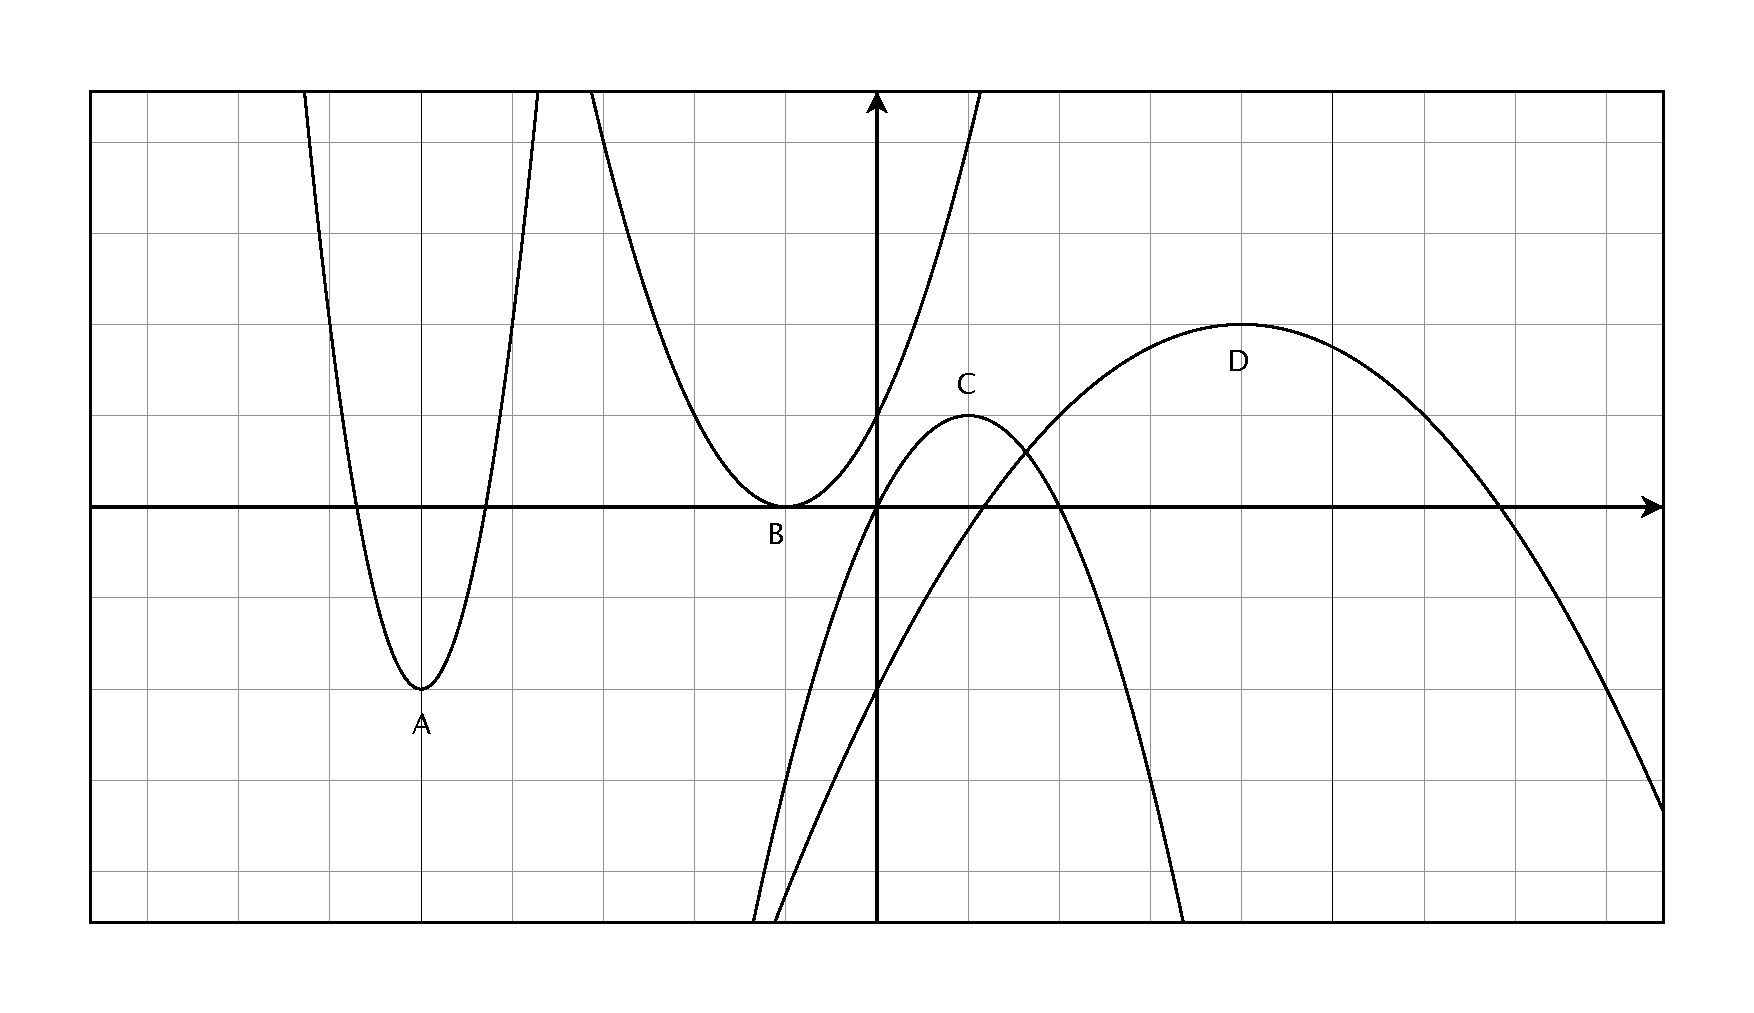
\includegraphics[scale=.3]{problem_7.eps}
%   \caption*{Problem 7}
% \end{figure}

% \begin{tabular}{cc}
% \toprule
% period & amplitude \\
% \midrule
%   $\pi$ & $2$ \\
% \bottomrule
% \end{tabular}

\title{Math 141 Notes \\ Section 4.5}

\date{July 3, 2013}

\begin{document}

  \maketitle
  \tableofcontents

  \section{Homework}
  \begin{enumerate}
    \item
      \[
        \ln 3x^2 = \ln 3 + 2 \ln x \neq 2 \left( \ln 3 + \ln x \right)
      \]
      Only $x$ is squared.

    \item $\log_a a = 1$

  \end{enumerate}

  \section{Population Growth}

  \subsection{Description}
  Just like compound interest: $n(t) = n_0 e^{rt}$.

  \begin{itemize*}
    \item $n$ population at time $t$
    \item $n_0$ initial population
    \item $r$ growth rate
    \item $t$ time
  \end{itemize*}

  \subsection{Examples}

  \begin{enumerate}
    \item bacteria with:
      \begin{itemize*}
        \item $n_0 = 1,000$ 
        \item $r = \unit[0.3]{hr}$ 
      \end{itemize*}

      \begin{enumerate}[a]
        \item find the function 
          \[
            n(t) = 1,000 e^{0.3 t}
          \]

        \item how many bacteria after 5 hours? 
          \[
            n(5) = 1,000 e^{0.3 \cdot 5} \approx 4,482
          \]

        \item how many bacteria after 24 hours? 
          \[
            n(24) = 1,000 e^{0.3 \cdot 24} \approx 1,339,430
          \]

        \item how many bacteria were present 2 hours ago? 
          \[
            1,000 = n_0 e^{.3 \cdot 2} \approx 549 
          \]

        \item how many bacteria were present 24 hours ago? 
          \[
            1,000 = n_0 e^{.3 \cdot 24} \approx 1 
          \]

      \end{enumerate}

    \item 2,000 bacteria; the population doubles every 3 hours
      
      \begin{enumerate}[a]
        \item find the rate:
          \begin{align*}
            2n_0 & = n_0 e^{3r} \\
            r    & = \frac{\ln 2}{3} \\
                 & \approx 0.231 \\
          \end{align*}

        \item how many after 2 hours?
          \[
            n(1) = 2,000 e^{0.231 \cdot 2} \approx 3,175
          \]

        \item when will there be 20,000?
          \begin{align*}
            20,000 &= 2,000 e^{0.231 t} \\
            t &\approx \unit[9.97]{hr} \\
          \end{align*}

      \end{enumerate}
      
  \end{enumerate}

\end{document}
